\documentclass[titlepage]{article}
\usepackage{fullpage}
\usepackage{graphicx}

\title{Enhancing the SP2 Framework with Virtual Memory and Separation of
       Kernel and User Programs}
\author{Garrett Smith, Alex Merritt\\
{\small Rochester Institute of Technology, Rochester, NY}\\
{\small \{gcs2980,amm1747\}@rit.edu}}
\date{\today}

% Some useful VIM commands:
% - select block of text, 'gq' remolds the paragraph
% - 'za' expands/collapses sections

% Latex stuff
% - \verb|code| is inline
% - \begin{verbatim} starts a block

\begin{document}

\maketitle
\newpage

\tableofcontents
\newpage

\listoffigures
\newpage

%
% Kernel-level Debugging with QEMU and GDB
%

\section{Kernel Level Debugging with QEMU and GDB}

A number of modifications have been made to the framework build system to
facilitate easier debugging and incremental development and testing. One of the
most useful enhancements is support for testing under an emulated x86 environment
using QEMU, an open source machine emulator. As QEMU supports hardware
virtualization (using KVM, the Kernel-based Virtual Machine), it provides a
secure virtual execution environment that is both highly accurate and capable of
near native speeds.

QEMU implements a gdb-stub, making it possible for gdb to connect to the 
emulator through a remote debugging session. Three new pseudo-targets have been
added to the Makefile to pass the necessary parameters to QEMU and set up the
debugging environment.

\begin{itemize}
\item \textbf{qrun} - builds the target image, then immediately executes the
    image under QEMU, redirecting the virtual serial interface to standard out
\item \textbf{qruns} - builds and loads the target image into QEMU, first
    invoking the telnet command to handle I/O over the virtual serial interface
\item \textbf{qdbg} - builds and loads the target image into QEMU, halting on the
    first instruction to execute, then invokes a remote debugging session under
    GDB
\end{itemize}

When entering a debugging session, GDB will begin halted at address
\verb!0xFFFF0!, the start of the BIOS initialization code. While it is possible
to step through the system initialization, it is not particularly useful. It is
more practical to break at the first instruction of either the bootstrap
program, or the kernel startup code. This can be achieved by issuing a
\textbf{break} command at addresses \verb!0x7C00! or \verb!0x10000!,
respectively.

For rudimentary instruction-level debugging, GDB must be told whether the system
is currently executing in 16-bit real mode, or 32-bit protected mode. This is
necessary for GDB to be able to properly interpret the opcode at the current
instruction address and display the correct mnemonic and instruction operands.
This task can be simplified through the use of a startup script. If present, GDB
will load and execute a \verb!.gdbinit! startup script. The script provided
contains three new commands for controlling the current
debug mode.

\begin{itemize}
\item \textbf{rmode} - sets the architecture to 16-bit real mode, displays
    the current instruction for each \textbf{next} command
\item \textbf{pmode} - sets the architecture to 32-bit protected mode, displays
    the current instruction for each \textbf{next} command
\item \textbf{cmode} - sets the architecture to 32-bit protected mode, disables
    instruction display (default mode for high level language debugging)
\end{itemize}

In addition to the command declarations, the provided \verb!.gdbinit! script,
upon startup, sets the default execution mode to 'rmode', loads symbolic
debugging information from the kernel object file (this requires invoking gcc
with the -gstabs flag, which may be enabled or disabled within the Makefile),
then attaches to the remote debugging session at \verb!localhost:1234!, the
default session host and port set by QEMU.

If debugging symbols are present in the kernel object file, GDB can be
controlled in the same way as one would debug a typical C or C++ application.
Note that the object file (kern.o) fed to GDB is separate from the final disk
image, which is a flat binary stripped of any debugging symbols or file/segment
headers (ELF or a.out).

As an alternative to interactive debugging, the build process has also been
modified to invoke \textbf{objdump} to generate a listing file for the kernel
image, which contains high level C-code inline with the disassembled image. It
is important to keep in mind that while running the framework under QEMU and GDB
is a far more pleasant experience than trial-and-error debugging on hardware,
modified code should be frequently tested and verified on real hardware. In
certain instances code that runs under QEMU may fail on systems in the
Distributed Systems Lab.

\begin{figure}[!ht]
The following code demonstrates a typical debugging session under GDB:
\begin{verbatim}
    rmode               # set real mode instruction decoding (set by default)
    break *0x7C00       # insert breakpoint at start of bootstrapping code
    continue            # skip over the BIOS startup code until the bootstrap
    ni                  # execute the first instruction of the bootstrap code

    pmode               # change from real mode to protected mode decoding
    break *0x10000      # insert breakpoint at kernel entrypoint
    continue            # skip over the bootstrap until the kernel entrypoint
    ni                  # execute the first instruction of the kernel startup

    cmode               # change from instruction-level to high-level mode
    break _init         # insert a breakpoint at the top of function '_init'
    continue            # skip over the startup until the _init function
    next                # execute a single line of (C-language) code
\end{verbatim}
\caption{QEMU/GDB Debugging Session}
\end{figure}

%
% Virtual Memory Using Pure Segmentation
%

\section{Virtual Memory Using Pure Segmentation}

\textit{All the information in this section is described in detail in the Intel
Manual Vol 3A.}

\subsection{Brief Overview of Virtual Memory}
A \textbf{physical address map} is a mapping of a range of addresses to physical
memory.  A \textbf{virtual address map} is a mapping of a collection of address
ranges onto a physical address map. Physical addresses are controlled by the
hardware, and virtual addresses by the kernel of an operating system with some
assistance from the hardware. Programs that run without the use of virtual
memory are able to read from and write to any address in memory simply by
referencing one, like so: \verb|*(0xACCE55ED) = 0xDA7A|. Since the address
\verb|0xACCE55ED| is a physical mapping, it is accessible to any and all
programs.

\begin{center}
    \begin{tabular}{c c c}
        Program & Program Address Space & Physical Address Space \\
        \hline
        process A & \verb|0x00000000-0xFFFFFFFF| & \verb|0x00000000 - 0xFFFFFFFF| \\
        process B & \verb|0x00000000-0xFFFFFFFF| & \verb|0x00000000 - 0xFFFFFFFF| \\
    \end{tabular}
\end{center}

With virtual memory---segmentation specifically---the kernel of an operating
system prevents virtual addresses from mapping to the same physical address, so
that no two addresses actually refer to the same location in physical memory.
When two programs refer to the same virtual address, it gets mapped to a
location within their respective physical mappings.  If for example, two
programs refer to address \verb|0x00000000| they might separately map to
\verb|0x02A00000| and \verb|0x05300000|:

\begin{center}
    \begin{tabular}{c c c}
        Program & Program Address Space & Physical Address Space\footnote{Assume a
        segment size of 1MB.} \\
        \hline
        process A & \verb|0x00000000-0x00100000| & \verb|0x02A00000 - 0x02B00000| \\
        process B & \verb|0x00000000-0x00100000| & \verb|0x05300000 - 0x05400000| \\
    \end{tabular}
\end{center}

Here's how the Intel Manual describes segmentation:

\begin{quote}\ldots segmentation provides a mechanism for dividing the
    processor's addressable memory space (called the \textbf{linear address space})
    into smaller protected address spaces called \textbf{segments}. Segments can be
    used to hold the code, data, and stack for a program or to hold system data
    structures (such as a TSS or LDT). If more than one program (or task) is running
    on a processor, each program can be assigned its own set of segments. The
    processor then enforces the boundaries between these segments and insures that
    one program does not interfere with the execution of another program by writing
    into the other program's segments. \ldots (Intel Vol. 3A Section 3.1)
\end{quote}

% 
% Segmentation Structures
%

\subsection{Segmentation Structures}

Translation of virtual addresses to physical addresses is accomplished via
\textbf{segment registers} and \textbf{segment descriptors}, the latter located
either in the \textbf{Global Descriptor Table} (GDT) or in one of many
\textbf{Local Descriptor Tables} (LDT).

\paragraph{Segment Descriptor}
A segment descriptor describes a contiguous block of physical memory---base
address, size, access rights, type, etc. These are eight bytes in size on the
32-bit machines in the DSL. The memory regions they describe can either be used
as raw memory (code/data) or hold system segments such as an LDT or TSS.
Descriptors can be found in the GDT as well as the LDT, and are referenced by
segment registers in the hardware (via an index into either table, not a direct
reference). The bit layout can be found in the Intel Manual Vol. 3A Section
3.4.5.

\paragraph{Descriptor Tables}
The Global and Local Descriptor Tables are contiguous chunks of physical memory
that contain 8-byte descriptors. In the framework, the GDT is defined and
created in \verb|bootstrap.S| at the label \verb|start_gdt|. LDTs act like GDTs
except that they are pointed to by descriptors in the GDT, using \textit{system}
segment descriptors, as opposed to \textit{data/code} segment descriptors---see
the \textbf{S flag}. In the framework each process that runs gets its own LDT
with two descriptors of its own (one for code and one for data), with a single
reference to the LDT in the GDT. Upon one of the task creation/modification
system calls (\verb|fork, exec*|) or a context switch the dispatched process'
LDT and LDT register contents get loaded (see Figure \ref{isr-restore}).

\paragraph{Segment Registers}
Segment registers contain segment selectors (abbreviated \textit{SS}), which are
16 bits wide and are composed of three parts: an \textit{index}, a \textit{table
indicator} and a \textit{request privilege level}. The index is an offset into a
descriptor table, where TI indicates which table to use (LDT or GDT). RPL isn't
used in the framework as all code runs with privilege level zero.  Segment
registers consist of \verb|ss, cs, es, ds, gs, fs| in addition to the
task-segment register (TSR) and the LDT register (LDTR). The GDT register is
\textit{not} a segment register, as it does not index itself (it holds the base
and offset of the GDT in physical memory, which all other segment registers
depend on).

In \verb|bootstrap.h| the macros
\verb|GDT_LINEAR, GDT_CODE, GDT_DATA, GDT_STACK| are the values stored in the
segment registers (the segment selectors) for the kernel which runs in linear
address space.

\begin{figure}[!ht]
    \centering
    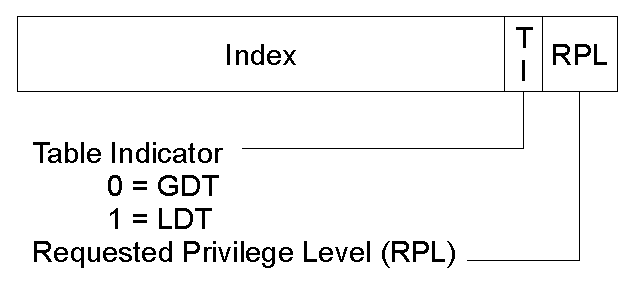
\includegraphics[width=0.35\textwidth]{images/segment_selector.eps}
    \caption{Segment Selector/Register Bit Layout}
\end{figure}

For example, a value of \verb|0x10| for \verb|GDT_CODE| means that the code
segment descriptor is the fourth descriptor inside the GDT, accessed using
privilege level zero (you can confirm this by looking inside \verb|bootstrap.S|
where the GDT is defined). This value would be inserted into the code segment
register \verb|cs| to tell it where in memory the segment is in which code to
execute is located.

Since all LDTs in the framework have no more and no fewer than two descriptors
which never change their index, the segment selectors for the LDTs are similarly
defined (see \verb|gdt_support.h|). Both point to indexes 0 (\verb|ldt_t.dseg|)
and 1 (\verb|ldt_t.cseg|)---\verb|0x4| and \verb|0xC|, respectively---inside the
currently-set LDT, again with privilege level zero.

\begin{figure}[!ht]
\begin{verbatim}
    typedef struct pcb {        typedef struct segment_s {  typedef struct physblock_s {
        Context *context;           physblock_t mem;            addr_t offset;
        Stack *stack;               ldt_t   ldt;                addr_t length;
        Time wakeup;                u32_t   ldtr;           } physblock_t;
        Pid pid;                } segment_t;
        Pid ppid;
        State state;            struct ldt_s {
        Priority prio;              gdt_entry_t dseg;
        segment_t seg;              gdt_entry_t cseg;
    } Pcb;                      } ldt_t;
\end{verbatim}
\caption{Example PCB Configuration}
\end{figure}

Each \verb|segment_t| object inside a process' PCB contains information
needed to make use of LDTs and segmentation. Context switching causes
\verb|ldtr| to be reloaded, along with the segment registers inside
\verb|Context|. Something to take note of is a second copy of \verb|ldtr| inside
\verb|Context|. This exists to allow pretty-printing of this register upon any
invocation to \verb|isr_save| in \verb|isr_stubs.S| (the upper-half of the
screen, where all registers are visible).

% 
% Initialization and Use
%

\subsection{Initialization and Use of Structures}

There is one trick to understand before assigning values to the segment
registers: they don't just store 16 bits of data, but contain \textit{hidden
bits} that are not visible to the programmer. Each and every time the value in
one of these registers changes the hardware will immediately use the stored
index and TI to look up the descriptor pointed to by this register, making a
local copy---these are the \textit{hidden bits}. This is important to know,
since \textit{General Protection Faults} can arise from loading the segment
registers without having created or initialized segment descriptors, the GDTR or
LDTR.

All members of \verb|segment_t| must be initialized before the process can be
dispatched. When \verb|mem| is hardcoded to \verb|0x0| and \verb|0xFFFFFFFF|,
and both descriptors in \verb|ldt_t| copied from the GDT, then those processes
are labeled ``kernel processes'' and do not actually run in their own segments,
but share those given to the kernel itself. Only two programs are allowed this,
\verb|idle_main| and \verb|first_main|. All other programs run separate from the
kernel space and in their own segments. View the code in the fork or exec system
calls to study how these are initialized. Note: \verb|mem| holds the address to
the region of memory designated as the segment. Technically only one segment
exists for a process, where the code and data descriptors overlap each other.

\begin{figure}[!ht]
    \centering
    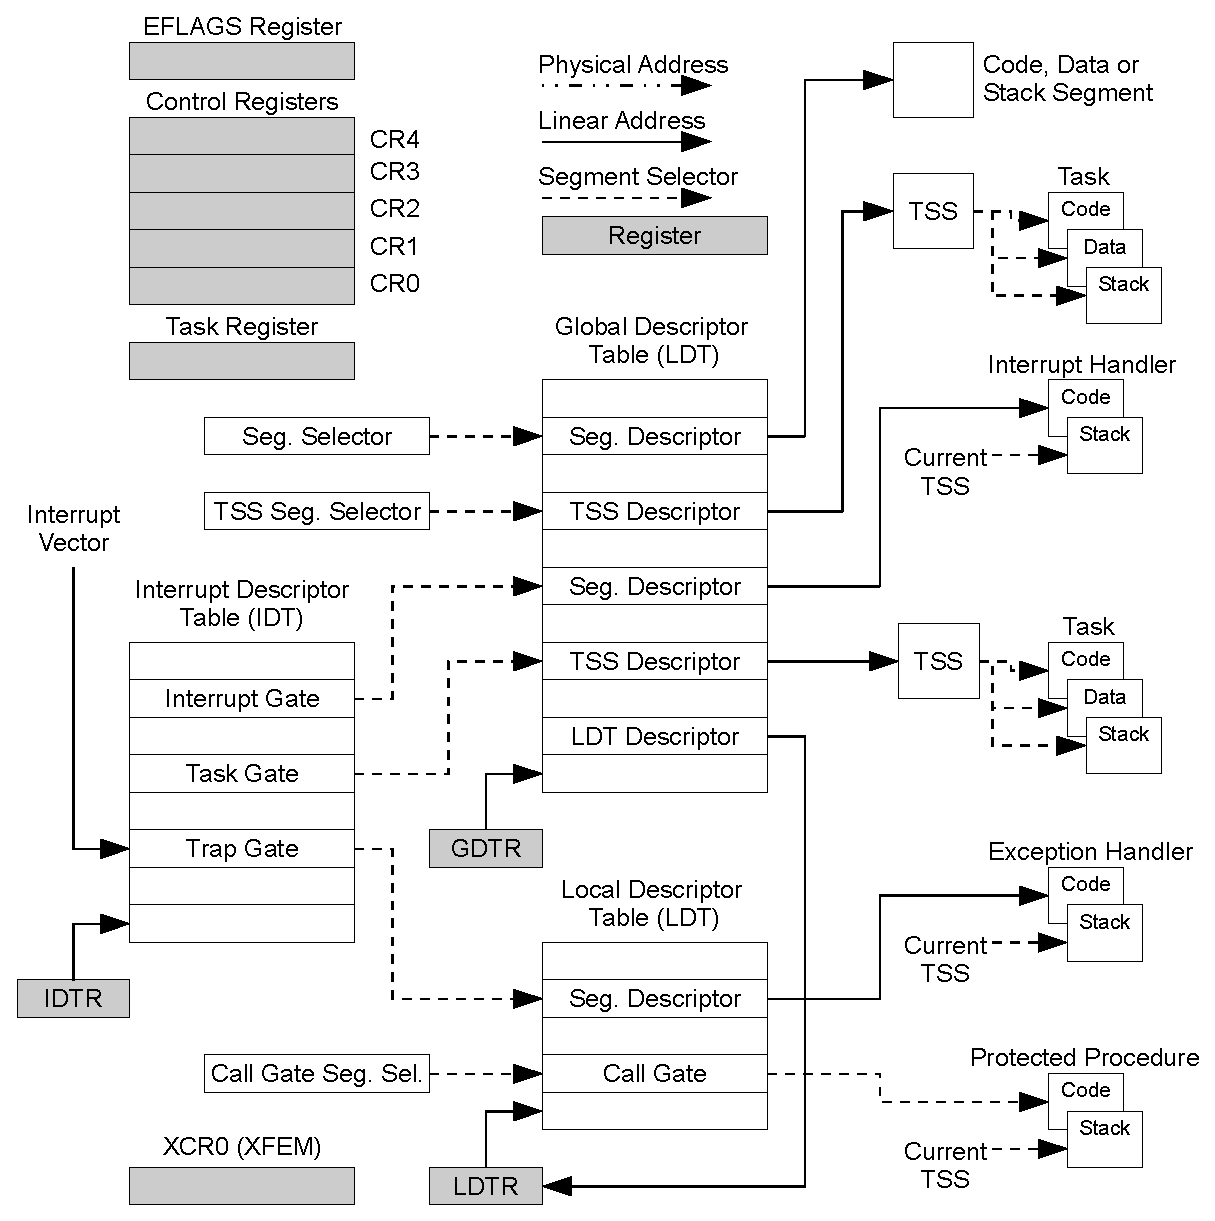
\includegraphics[width=0.70\textwidth]{images/structures.eps}
    \caption{Segment Structures and Functions.}
\end{figure}

\paragraph{Accessing a Segment Descriptor} If the TI bit in the segment register
indicates GDT, the physical base address of the GDT (taken from the GDTR) is
added to the product of the index and eight---the size of a descriptor.  If the
TI bit is set to indicate LDT use, the index in the segment register points not
to an offset in the GDT but in the LDT. The descriptor of the LDT itself is
pointed to by the index inside the LDTR which, as mentioned above, is a segment
register itself. Once the base address of the LDT is established, it is used to
access the descriptor via the index inside the segment descriptor.

\begin{figure}[!ht]
    \centering
    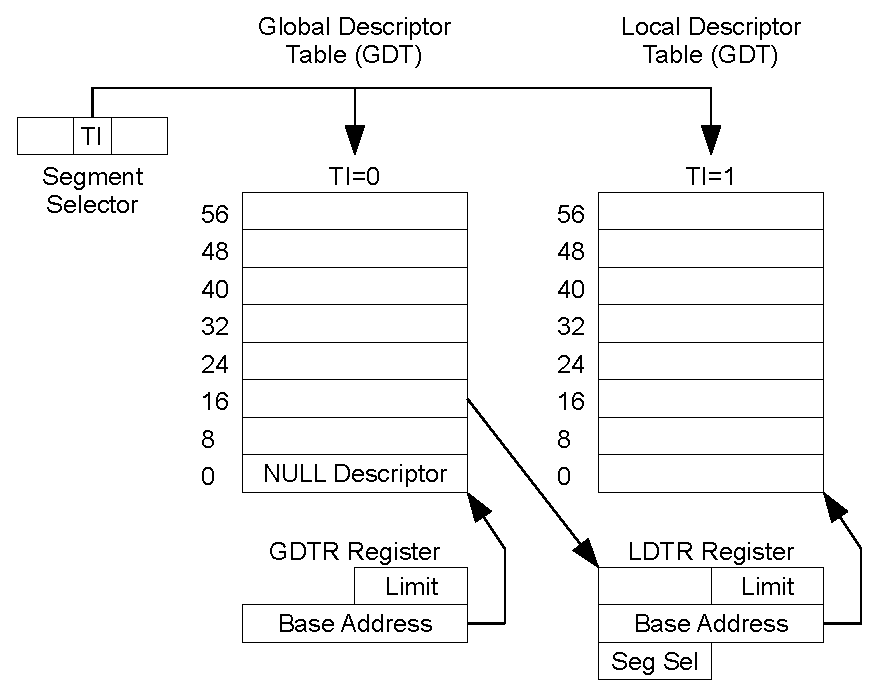
\includegraphics[width=0.55\textwidth]{images/descriptor_tables.eps}
    \caption{Local and Global Descriptor Tables.}
\end{figure}

\newpage
Restoring the context requires a bit of hard-coding and clever thinking to
access the components in a Pcb.

\begin{figure}[!ht]
\begin{verbatim}
    // Restoring the context
    subl    20(%ebx), %esp      // 1. translate stack addr back to virtual address
    movl    44(%ebx), %eax      // 2. Restore LDTR
    lldt    %ax                 // Must be done before loading any segment selectors.
    movl    $4, %eax            // 3. Restore SS = LDT_DSEG = 0x4
    movl    %eax, %ss           // NOTE: If LDT_DSEG changes, this must too!
    popl    %[sgfesd]s          // restore the segment registers
    popl    %eax
    popa
    addl    $8, %esp
    iret
\end{verbatim}
\caption{Modifying $isr\_stubs.S:\_\_isr\_restore$}
\label{isr-restore}
\end{figure}

\begin{enumerate}
    \item Physical addressing must become virtual again to allow the user
    processes to continue executing. Here, \verb|20(%ebx)| $\equiv$
    \verb|Pcb.seg.mem.offset|
    \item This step must now access \verb|ldtr| of the next context. Since this
    code is heavily dependent upon the layout and contents of the Pcb, offset 44
    must change if the Pcb does. Here, \verb|44(%ebx)| $\equiv$
    \verb|Pcb.seg.ldtr| Note: even though \verb|ldtr| is 32 bits wide, the
    register is only 16 (thus loading \verb|ax| instead of \verb|eax|).
    \item Load the segment registers with the appropriate segment selectors. As
    mentioned above, these values are static. We must set \verb|ss|
    appropriately in order to access the stack segment onto which the context
    was pushed.
\end{enumerate}

Again, keep in mind that the last lines (above) that load the segment registers
automatically access the GDT, LDT, GDTR, and LDTR to load the hidden bits of
those registers.  If the structures are not set up correctly, any one of these
lines can throw a General Protection Fault.

\subsection{Why Segmentation?} Segmentation existed before paging, and
was---at the time---the best and most appropriate solution to solve many issues.
Now that we have paging, segmentation is really a step back in time for those
who choose to implement it, if they have the option for full paging support.

Segmentation was chosen as the medium for virtual memory, as it would not take
paging away as an individual project for Systems Programming 2. As it is older
technology and paging newer, an implementation of paging would be more
worth-while to get working.

\begin{figure}
\begin{tabular}[c]{l l l}
                        &   Segmentation    & Paging    \\
\hline
Programmer Awareness    & Yes       & No                \\
Compilation             & Separate  & Not separate      \\
Linear Address Spaces   & 1         & Many              \\
Device I/O              & Port-based& Port-based or Memory-mapped \\
Why Invented?           & division; protection; sharing & Increase address space \\
\end{tabular}
\caption{Differences Between Segmentation and Paging}
\end{figure}

Implementing shared memory in the framework with the current support of
segmentation is not easy. Since the GNU compiler is not segmentation-aware
(meaning it assumes a flat address space), accessing data in another segment
involves changing the segment registers. This requires assembly, as there is no
statement in C to access those registers. Moving data across program address
spaces would involve copying data across segments, requiring segment registers
to be modified multiple times, via system calls. With paging, a physical address
space is simply mapped by a virtual address using the page tables, and those
shared addresses immediately become part of both process' address spaces.

Currently, the framework supports port-based I/O, which means calling functions
in order to access registers on devices, such as the serial port. Converting to
memory-mapped I/O would mean these ports could be transparently mapped to memory
addresses and handled as pointers to some address in memory. But, again,
accessing memory addresses outside of the currently-enabled segment involves
modifying the segment registers, which requires system calls defeating the whole
purpose.

64-bit architectures are phasing out support for segmentation altogether.
Porting the framework to this technology will require a rewrite of the virtual
memory support to use paging instead, without any segmentation.

\subsection{Incorporating Paging}

Two options currently exist for incorporating paging into the framework. There
also exist two framework code bases which can be used (the one this project was
based off of---no virtual memory---and this current one):

\begin{enumerate}
    \item Implement paging on top of the new framework. This option means that
    paging can only occur \textit{within} each of the segments instead of
    globally. Restrictions created from segmentation might not go away, such as
    trying to create memory-mapped I/O.
    \item Rework paging into the original framework as was done with
    segmentation in this project. This is acceptable, and the current framework
    may even be used a basis for a working implementation to get ideas from for
    how virtual memory works, which could be applied to paging.
\end{enumerate}

\subsubsection{Swapping}

Implementing swapping involves hardware, and subsequently writing a driver for
that hardware so that the framework has support to actually do the swapping to
that device (such as a hard disk). Furthermore, a decision will need to be made
as to whether segments or pages should be swapped to the storage medium.  Since
segments are contiguous chunks of physical memory (and need to be whole to
work), they cannot be split up, so entire segments will need to be moved around.
Currently, segments are 1MB in size. Moving that much data---most of which will
probably be empty---will take lots of time. Swapping works better with paging,
but that currently doesn't exist and would need to be incorporated into the
framework via the options above.

Getting swapping to work might not have any practical purpose, unless 1GB of
physical memory turns out to be inadequate, or if the systems upgrade to a newer
architecture.

\subsection{Task-State Segment}

Support for a Task-State Segment\footnote{See Intel Manual Vol. 3A Chapter 6}
(TSS) exists, but isn't actually needed. It works in combination with privilege
levels, which the framework does not take advantage of. Each physical processor
is assigned its own TSS, which is why there is currently only one, and assumed
to only be one. If the framework were to be modified to support one of the
dual-CPU machines in the lab, then a second TSS will need to be created and
assigned to the second chip.

\subsection{Memory Management}

A generic memory manager exists that is used to allocate segments for the
system. The code for this is located in \verb|segment.h| and \verb|segment.c|.
Function calls to manage contiguous blocks of memory are \verb|_phys_*()|, and
the functions to manage descriptors in the GDT are \verb|_gdt_alloc()| and
\verb|_gdt_alloc()|. The latter two return indexes into the GDT which can be
used to access descriptors in conjunction with \verb|g_gdt_table|---a reference
to the GDT in C. Since each process is assigned its own descriptor in the GDT,
the index returned by a call to \verb|_gdt_alloc()| is stored in
\verb|Pcb.seg.ldtr|. The former two manage physical memory, up to the 1GB
boundary. Think of them as \verb|malloc()| and \verb|free()|.

\section{Separating the Kernel and User Programs}

Prior to the implementation of segmentation and process address space
isolation, a "user program" was simply a function compiled and linked
directly into the kernel. Upon \verb!fork!ing, the new process was nothing
more than a separately scheduled thread of execution within the same kernel
image, with its own private stack and context block. As the same code and data
segments were shared between all running processes, there was no form of
protection shielding any one process from another. All non-stack data could
be altered by any of the running processes without any form of inter-process
synchronization.

While this system provides a simple and constraint-free environment to develop
and experiment within, it is a poor model of how real operating systems handle
process management. Despite the inherent flexibility of imposing no restrictions
on where and how user processes execute, it is ultimately a dangerous and
unpredictable system. 

\subsection{Initial (Naive) Implementation}

Each user processes is allocated its own (overlapping) code and data segments.
It is guaranteed that each processes' flat address space is contiguous and does
not overlap with the address space of any other running process. Given this
constraint (and, as per usual, limitations stemming from using pure segmentation
with a compiler that assumes a flat address space), no two processes share even
the same code segment. When a process \verb!fork!s, the calling process' address
space is copied, in its entirety, to the newly created process' address space.
The copy implementation is a fast, aligned memory blit from the source segment
to the destination segment. In addition to the newly allocated memory space and
segment descriptors, the child process is allocated a stack (which is a
reserved, fixed size block residing at the beginning of the process' segment)
identical to the calling process stack.

The subsequent call to \verb!exec! from the newly \verb!fork!ed process simply
initializes the process stack to a fresh state and begins execution at the
specified memory address. Very little actual work needs to be performed within
\verb!exec! for this particular implementation, given that the memory image is
not changed, just the instruction pointer of the process executing within it.

\subsection{Necessary Division Between User and Kernel Libraries}

While this implementation works, it introduces a number of new problems.
Although the address spaces of each user program are now truly separated from
one another (and more or less protected through the base offset and limit
fields), the entire kernel image and kernel library is duplicated within each
new process. Not only can the user programs make direct calls to kernel
functions, they will yield unexpected (and undesirable) results. For instance,
the console I/O routines write directly to the memory mapped VGA text buffer.
When the kernel invokes any of these functions from the physical address space,
each character is copied directly to an offset from physical address
\verb!0xB8000!, which will be reflected in the terminal. However, if a user
process executing within its own address space writes to memory location
\verb!0xB8000!, in actuality it is writing to physical address
\verb!SegmentOffset + 0xB800!.

Upon physically relocating each executing process, the division between what
tasks must be performed at the kernel level, and what tasks may be performed
by processes in execution becomes apparent.\footnote{Things stop working as
expected.} Resolving these issues (such as the console I/O failure above)
requires that a system call interface be established for any routines that may
only be performed within kernel space. Note that in this particular scenario
"kernel" and "user" space refers only to the distinction between parts of the
operating system executing within the flat, physical address space and the
parts executing within logical (segmented) regions of memory. User processes
still execute at the same privilege level (ring 0) as the kernel. In the case
of the console I/O routines, whereas previously user processes could make direct
calls to c\_puts and c\_putc, they must now invoke the puts and putc system
calls, trapping the operating system, which in turns dispatches the appropriate
routines on behalf of the calling process.

\begin{figure}[!ht]
    \centering
    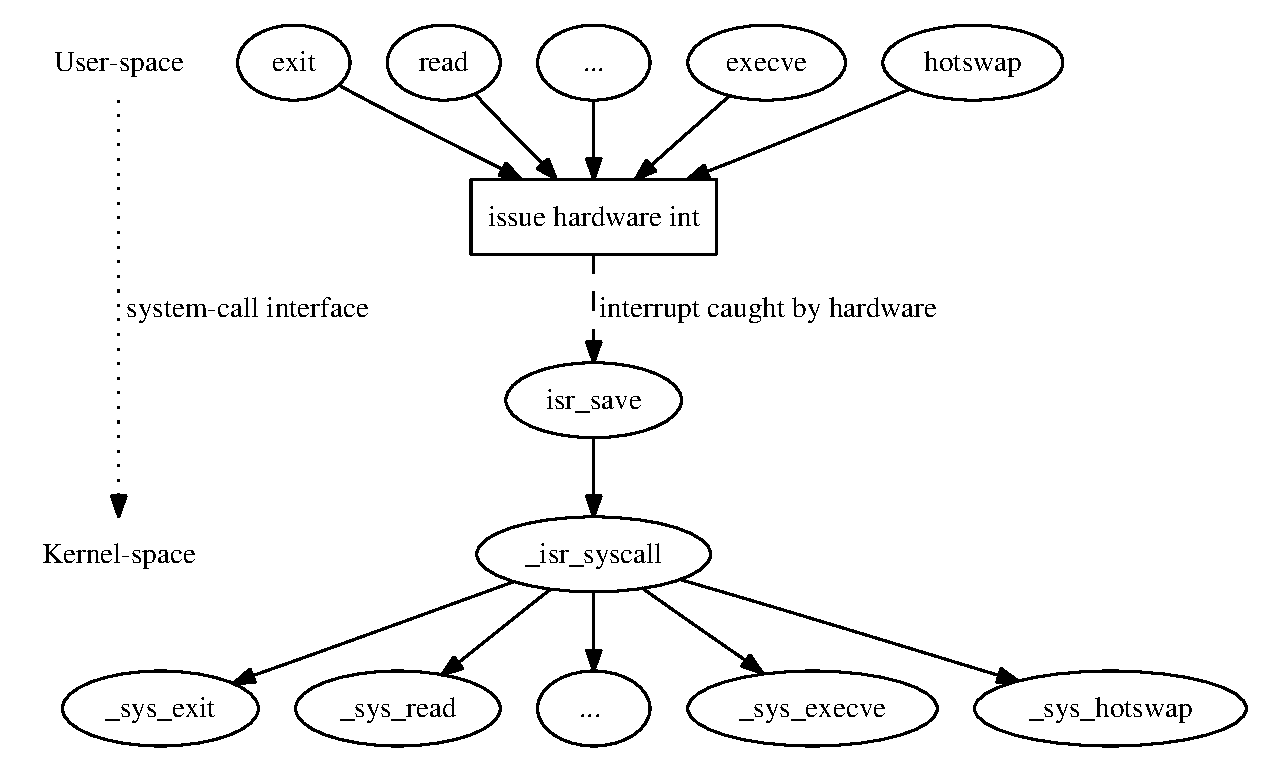
\includegraphics[width=0.8\textwidth]{images/interrupts.eps}
    \caption{Invoking System Calls via Interrupts.}
\end{figure}

\subsection{Loading Standalone ELF Executables}

With the aforementioned system call plumbing in place, this model is 
functionally correct. However, the "programs" are still functions within the
kernel, and they are still linked together with a mass of kernel symbols that
should not (and in most instances, cannot) be accessed directly. In addition to
separating the physical addresses of process execution space, each user program
should be compiled, linked, and loaded as a separate entity. While there
would be nothing fundamentally wrong with storing and loading user programs as
flat, stripped binaries (as is the kernel image), a more dynamic way to store
and load user programs is through a common, well supported executable file
format. This appraoch is more useful in the long run, given that I/O drivers
and file systems will eventually be built on top of the framework code.

The Elf32 file format is relatively simple to parse and load, and is the natural
choice given that the framework is built with the GNU toolchain. Thankfully,
the trickiest details of the specification have to do with linking and dynamic
relocation, which can be safely ignored, as we are only loading statically
linked executables. The block diagram below illustrates the high level
structure of an ELF executable from the loading and execution perspective.

\begin{figure}[!ht]
    \centering
    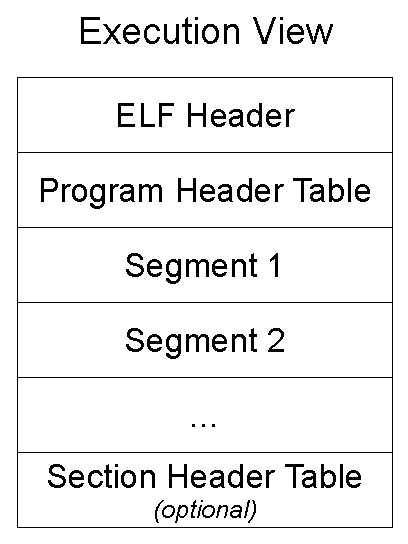
\includegraphics[width=0.20\textwidth]{images/elf_block.eps}
    \caption{ELF Executable Structure}
\end{figure}

From the ELF header block (Elf32\_Ehdr in the below code listing), the loader
verifies the object file identification fields and machine architecture. It
also obtains the virtual address of the program entrypoint from the
\verb!p_entry! field and the offset to the Program Header Table from the
\verb!p_phoff! field. This table describes one or more program segments to be
loaded into memory. The section headers can be safely ignored.

After verifying that the image is valid, the loader then iterates over each
program header block (Elf32\_Phdr  in the below code listing). There are a
number of different types of program headers, specified by the \verb!p_type!
field, but for a statically linked image only loadable (\verb!PT_LOAD!)
segments must be copied into mememory. The \verb!p_offset!  (file offset to
segment data), \verb!p_vaddr!  (load address in main memory), and
\verb!p_filesz! (segment size on disk) fields determine where the segment is
loaded, and how many bytes must be copied.

From the perspective of the application developer, the execution of a user
program begins at the \verb!main! function. However, before user program 
execution begins, pre-\verb!main! initialization must be performed. For this
simplified implementation, the initialization stub simply clears the BSS
(Block Started by Symbol) segment, calls the \verb!main! function, then finally
invokes the \verb!exit! system call (this allow standalone programs to terminate
with a \verb!return! statement from \verb!main! as opposed to an explicit call
to \verb!exit!). This process is similar to the kernel startup routine
(\verb!startup.S!). However, the kernel startup code contains additional
kernel-specific initialization and therefore can not be re-used. Each standalone
user program is linked to its own copy of the user startup code
(\verb!ustart.S!), which serves as its absolute entry-point (this is described
in detail in the next section).

\begin{figure}[!h]
\begin{verbatim}
    typedef struct {                                typedef struct {
        unsigned char   e_ident[EI_NIDENT];             Elf32_Word  p_type;
        Elf32_Half      e_type;                         Elf32_Off   p_offset;
        Elf32_Half      e_machine;                      Elf32_Addr  p_vaddr;
        Elf32_Word      e_version;                      Elf32_Addr  p_paddr;
        Elf32_Addr      e_entry;                        Elf32_Word  p_filesz;
        Elf32_Off       e_phoff;                        Elf32_Word  p_memsz;
        Elf32_Off       e_shoff;                        Elf32_Word  p_flags;
        Elf32_Word      e_flags;                        Elf32_Word  p_align;
        Elf32_Half      e_ehsize;                   } Elf32_Phdr;
        Elf32_Half      e_phentsize;
        Elf32_Half      e_phnum;
        Elf32_Half      e_shentsize;
        Elf32_Half      e_shnum;
        Elf32_Half      e_shstrndx;
    } Elf32_Ehdr;
\end{verbatim}
\caption{Relevant Elf32 Structures}
\end{figure}

\subsection{Updating the Build Process}

Each standalone user program need only be linked with the user startup routine,
user library routines, and the user portion of the system call interface. These
modules are ustart, ulibs and ulibc, respectively. The order of these object
files is important during the linking phase (the startup code must be linked
first). The necessary user object files are encapsulated within the
\verb!USER_OBJS! Makefile variable. As the framework initially contains no
support for I/O devices or file systems, the user programs used as an example
here are stored on disk immediately following the kernel, using the BuildImage
tool. During the bootstrapping phase each user program ELF is loaded to its
specified location in memory.

\begin{figure}[!ht]
\begin{verbatim}
    USER_OBJS = ustart.o ulibs.o ulibc.o
    USER_PROG = user1 user2 user3
    IMG_OBJS  = hswap.b 0x3000 kern.b 0x10000 user1 0x40000 user2 0x50000 user3 0x60000

    user1: $(USER_OBJS) user1.o
        $(LD) $(LFLAGS) -o user1 -s -Ttext 0x1000 $(USER_OBJS) user1.o

    user2: $(USER_OBJS) user2.o
        $(LD) $(LFLAGS) -o user2 -s -Ttext 0x1000 $(USER_OBJS) user2.o

    user3: $(USER_OBJS) user3.o
        $(LD) $(LFLAGS) -o user3 -s -Ttext 0x1000 $(USER_OBJS) user3.o

    floppy.image: bootstrap.b hswap.b kern.b kern.nl $(USER_PROG) $(UTILS)
        ./BuildImage -o floppy.image bootstrap.b 0x00 $(IMG_OBJS)
\end{verbatim}
\caption{Makefile - User Program Compilation}
\end{figure}

Note that the each user programs' text section begins at (virtual) address
0x1000. This is the address immediately following the process stack. This
approach was taken for the sake of simplicity. Prior to the introduction of
virtual memory, the framework allocated each process a fixed size stack in
the physical address space. Process stacks have been left at fixed sizes, but
have been moved into the process address space at offset 0x1000, growing down.
A better approach would be to start the stack at the very end of the segment,
so that code and data would grow up from offset 0, and stack would grow down
from address \verb!SegmentLimit!. However, as there is no current implementation
of dynamic memory in place, it is easier to simply fix the code and stack
at the start of the segment and assume everything from the end of the BSS to
\verb!SegmentLimit! is free for general purpose use.

\begin{figure}[!ht]
\begin{verbatim}
        char *pargs[] = {"user3", "user2"};
        int pid = fork();
        if (pid < 0) { /* error */ }
        else if (pid == 0) {
            execve(0x60000, pargs);
            exit();
        }
\end{verbatim}
\caption{execve Usage Example}
\end{figure}

A reference implementation of the \verb!execve! system call has been provided
to supplement the existing \verb!exec! routine. The new system call
takes the address where the executable will be loaded from memory, as well as
an array of string arguments that will be passed to the user program's
\verb!main! function. The code snippet above demonstrates one process, user2,
creating a new child process, user3, using the \verb!execve! system call.

\section{Booting the Kernel from USB Mass Storage Devices}

Using USB flash drives as a storage medium provides a number of advantages over
traditional floppy disks.

\begin{enumerate}
    \item solid state memory is far less prone to read/write errors
    \item increased durability and much longer expected lifetime (especially
    under the stress of repeated booting)
    \item faster read/write speeds (30 MB/s read, 15 MB/s write) compared to
    floppy disks (less than 125 KB/s)
    \item storage capacity largely increased (upwards 16GB compared to 1.44 MB)
    \item floppy disk drives are being phased out, whereas modern PCs typically
    have four or more USB ports
\end{enumerate}

Given that the added support for emulation and debugging under QEMU enables
development outside of the lab, as well as the decreasing likeliness that
typical laptop or desktop systems will come equipped with a floppy disk drive,
it is necessary to modernize the boot process. USB booting is the fastest and
most straightforward of the available options.

\subsection{Requirements for USB Boot}

Booting from a USB flash drive requires that the PC BIOS supports USB boot, as
well as that the flash drive itself is boot-capable. All of the systems
available for use in the Distributed Systems Lab appear to be capable of USB
boot in addition to booting from traditional storage devices.

From the perspective of the operating system, or more specifically, the boot
strapping code, the BIOS exposes the USB drive to the system (through
\verb!int 0x13!, the Low Level Disk Services) as if it were a standard hard
disk drive.  Therefore, a bootstrap program that is already capable of loading a
kernel installed to a hard disk should be bootable from a USB drive without any
modifications. For each of the \verb!int 0x13! service routines, the caller
specifies the drive number using bits 0 through 6 of the DL register. If bit 7
is clear, the value indicates a floppy disk index. If bit 7 is set, the value
indicates a hard disk index.

Prior to these modifications, the bootstrap code only supported booting from
the first floppy drive (hard-coded to index 0, or drive A:). However, the 
modifications necessary to generalize boot device selection are relatively
minimal.

A more robust bootloader program, such as GRUB or LILO, might provide an
interactive boot menu or a configuration file to specify the boot device, or
provide separate bootstrap programs based on the loading mechanism (for
instance, a very simple floppy-based boot program that installs the kernel and
a more robust second-stage loader to the hard disk bootsector, then subsequent
boots from the hard disk immediately load and execute the second-stage boot
program). For the sake of simplicity, the modified framework boot program simply
loads the drive index from a memory location within the first-stage bootstrap
image.  This drive index is written to the disk image during the build process
using a slightly modified version of the BuildImage tool.

\subsection{Design and Implementation}

The BuildImage tool is used to construct the final disk image from one or more
(stripped) binary program files, in addition to the boot program. The updated
BuildImage takes the boot drive index as a command line argument and writes
it into the output disk image at location \verb!0x508! (one word before the
required first-stage boot signature \verb!0xAA55!. At runtime, the bootstrap
program loads this value and uses it as the device index parameter for each
\verb!int 0x13! service call.

Depending on the \verb!make! target, the build system creates one of two
targets, \verb!floppy.image! or \verb!hdrive.image!. The \verb!make! targets
are \verb!floppy! and \verb!flash!, respectively. The two images are constructed
with BuildImage in the following manner:

\begin{verbatim}
    ./BuildImage -o floppy.image bootstrap.b 0x00 $(IMG_OBJS)
    ./BuildImage -o hdrive.image bootstrap.b 0x80 $(IMG_OBJS)
\end{verbatim}

Whereas one can assume the first floppy disk device to be mapped to the special
file /dev/fd0, USB device file names are less consistent between various flavors
of UNIX. To counter this problem, the Makefile determines the floppy device file
path from the environment variable \verb!USB_DEV!. Images are built as follows:

\begin{verbatim}
    make floppy                         # assumes floppy at /dev/fd0
    sudo USB_DEV=/dev/sdd make flash    # USB at /dev/sdd
\end{verbatim}

\section{Implementing a Quick "Warm-Boot" Mechanism}

Despite the numerous advantages of developing and debugging system software
under emulation, it is still necessary to verify its correct functionality on
real hardware. Often, for a variety of different reasons, some piece of code may
work under the emulator, but fail on hardware. In this scenario it is necessary
to revert to the build-copy-boot-repeat cycle of testing on the lab machines.
Even with USB boot it can be frustrating to repeatedly sit through the lengthy
BIOS startup routines and splash screens.

To get around these delays, it is possible to soft-reset the system, avoiding
the full-blown system initialization of a cold boot. However, reloading the
bootstrap program (and, in turn, the new kernel) requires support for reading
from an I/O device. After switching into 32-bit protected mode, this requires
developing a device driver (for either the floppy disk controller or ATA hard
disk controller). Developing such a driver would be beyond the scope of this
project, and as both are fairly obvious choices for a student project, they do
not belong in the bare framework.

\subsection{Switching from Protected to Real Mode}
The simple solution to this problem is to temporarily revert back to 16-bit real
mode, so that the disk I/O can be performed using the BIOS interrupts
(\verb!int 0x13!). While this may not optimal, it is the only solution available
in the absence of real drivers.  However, the switch from protected mode back to
real mode is not as trivial of an operation as simply clearing the Protected
Environment flag (bit 0) of the base Control Register (CR0). Section 9.9.2 of
the Intel System Programming Guide (Volume 3A) lays out the necessary steps
required to perform a successful mode switch:

\begin{enumerate}
    \item disable interrupts using the CLI instruction
    \item if paging is enabled, additional operations must be performed
    (excluded for segmentation model)
    \item program control must be transferred to a pseudo 16-bit code segment
    (has an address limit of 64 KB)
    \item data segments SS, DS, ES, FS and GS must be set to valid pseudo 16-bit
    data segment selectors (address limit of 64 KB, byte granular, expand up,
    writable, present)
    \item segment registers loaded with the null segment will be unusable in
    real mode, segment registers that are not reloaded prior to the switch will
    continue using the attributes loaded for protected mode execution
    \item load the interrupt descriptor table (IDT) register with an address
    within the 1 MB address range
    \item clear the PE flag (bit 0) of the CR0 register to switch to real mode
    \item perform a long jump to the first real mode instruction to execute,
    this is necessary to flush the instruction queue and reload the CS register
    (which is 0, as the segment registers now specify a base address as opposed
    to a descriptor offset)
    \item reload the SS, DS, ES, FS and GS to the necessary base addresses
    \item re-enable interrupts using the STI instruction
\end{enumerate}

\subsection{Design and Implementation}

The remaining challenge lies in placing the real mode "hotswap" program in
memory. As soon as the program begins executing in real mode, the instruction
pointer must be at a valid 16-bit real mode address (as the long jump will reset
the base address to 0, this must be within the 65 KB boundary). Since the kernel
will be loaded and executed at address \verb!0x10000! (just beyond the limit),
the real mode program cannot be linked in with the kernel image.

To get around this problem, the real mode "hotswap" program (hswap.b) is built,
linked, and loaded separately from the kernel. The swap image is loaded into
a guaranteed valid (and unused) region of low memory using the BuildImage tool.
The system call that performs the swap is just small block of inline assembly
that jumps to the address where the hswap.b was loaded (RMTEXT\_ADDRESS, which
in this case happens to be \verb!0x3000!).

hswap.b, once switched into real mode, displays a prompt requesting the user
to select the boot device (either floppy or HDD/flash). Once a valid response
is obtained, the first sector (512 bytes) of the boot device is loaded at
address \verb!0x7C00!. The program then jumps to this address, and the bootstrap
process is repeated using the new image.

\begin{figure}[!ht]
\begin{verbatim}
        [Real Mode Boot Menu]


        0 - [0x00] Floppy Drive A
        1 - [0x01] Floppy Drive B
        2 - [0x80] Hard Disk 0
        3 - [0x81] Hard Disk 1

        Select boot device [0x80]:
\end{verbatim}
\caption{Displayed Boot Menu Prompt}
\end{figure}

Unfortunately the DSL machines do not appear to recognize bootable USB devices
through the system services once the device has been removed or inserted 
following system startup. As a result this functionality is limited to floppy
disks for lab machines. However, other motherboards and BIOS versions tested
outside of the lab had no problems detecting and booting from flash drives
inserted after boot.

\section{Resources}
Books:
\begin{itemize}
    \item Intel 64 and IA-32 Architectures Software Developer's Manual Volume 3A
    \item System V Application Binary Interface, Edition 4.1
    \item Operating Systems Design and Implementation, Andrew S. Tanenbaum
\end{itemize}
Online:
\begin{itemize}
    \item OSDev.org, http://www.osdev.org
    \item The Operating System Resource Center,
          http://www.nondot.org/sabre/os/articles
\end{itemize}
\end{document}

